\documentclass[border=3pt]{standalone}
% Preâmbulo compartilhado pelos diagramas TikZ da aula 14 (SLAM com EIF)
\usepackage[T1]{fontenc}
\usepackage[utf8]{inputenc}
\usepackage{lmodern}
\usepackage{amsmath}
\usepackage{xcolor}
\usepackage{tikz}
\usetikzlibrary{arrows.meta,angles,quotes,decorations.pathmorphing,decorations.pathreplacing,calc,
                positioning,shapes.geometric,shapes.misc,backgrounds,fit,
                math}

% Paleta (mesma dos SVGs originais)
\definecolor{dblue}{HTML}{2A5B8C}
\definecolor{dorange}{HTML}{B3541E}
\definecolor{dgreen}{HTML}{4A7C59}
\definecolor{dred}{HTML}{9C4B4B}
\definecolor{dcream}{HTML}{F4F1EA}
\definecolor{dshade}{HTML}{DDD7C9}

% Função gaussiana (não normalizada por padrão de escala visual)
\pgfmathdeclarefunction{gauss}{3}{%
  \pgfmathparse{1/(#3*sqrt(2*pi))*exp(-((#1-#2)^2)/(2*#3^2))}%
}

% Estilos comuns (prefixo d... para não colidir com chaves internas do pgf)
\tikzset{
  >={Stealth[length=2mm]},
  dguide/.style={gray!55, dashed, line width=0.4pt},
  daxis/.style={gray!60, line width=0.7pt, ->},
  dbody/.style={fill=black!3, draw=black!80, line width=1pt},
  dacc/.style={draw=dblue, line width=1pt},
  dlbl/.style={black!55, font=\small},
  dsub/.style={black!45, font=\footnotesize},
  dstate/.style={circle, draw=black!80, fill=dcream, line width=1pt,
                 minimum size=17mm, font=\large, inner sep=1pt},
  dobs/.style={circle, draw=black!80, fill=dshade, line width=1pt,
               minimum size=14mm, font=\large, inner sep=1pt},
  dbox/.style={rounded corners=2pt, draw=black!80, fill=dcream, line width=1pt,
               align=center, inner sep=6pt},
  dop/.style={circle, draw=black!80, fill=white, line width=1pt,
              minimum size=6mm, inner sep=0pt, font=\small},
  dtrans/.style={->, dblue, line width=1pt},
  dmeas/.style={->, dorange, line width=1pt},
  dcurve/.style={line width=1pt, dblue},
  dcurveb/.style={line width=1.4pt, dorange},
}

\begin{document}
\hyphenpenalty=10000 \exhyphenpenalty=10000 \tolerance=9999 \emergencystretch=3em
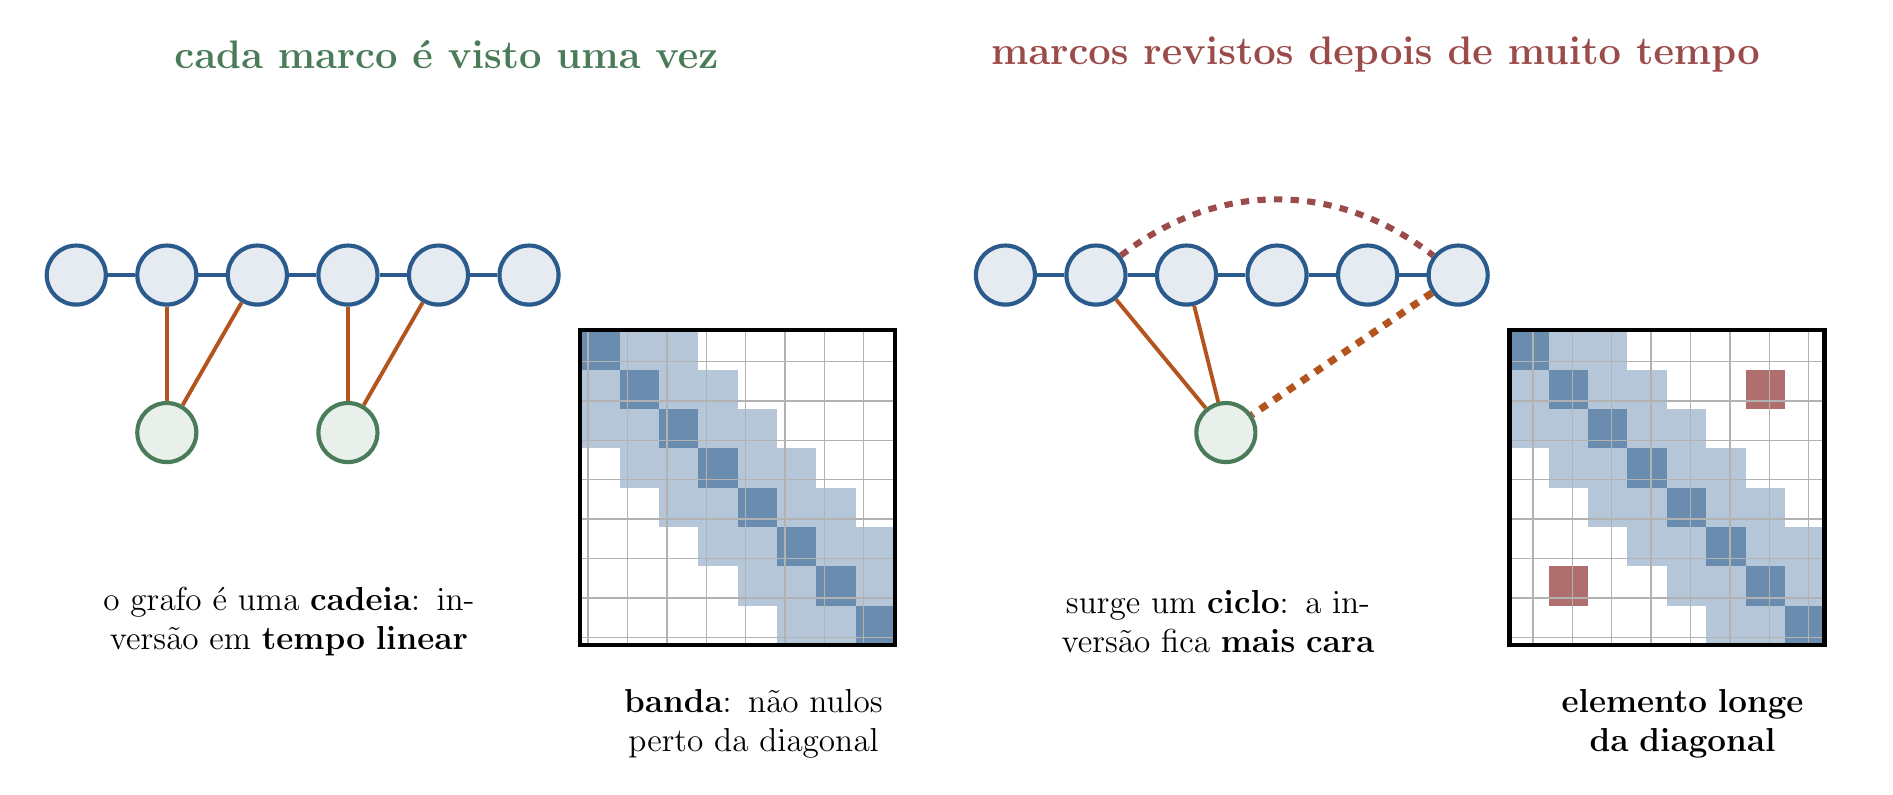
\begin{tikzpicture}[x=1cm,y=1cm]
\tikzset{p/.style={circle, draw=dblue, fill=dblue!12, line width=1.5pt, minimum size=0.75cm},
        m/.style={circle, draw=dgreen, fill=dgreen!12, line width=1.5pt, minimum size=0.75cm}}
\node[font=\Large\bfseries, text=dgreen] at (5.2,8.4) {cada marco é visto uma vez};
\node[p] (ap0) at (0.5,5.6) {};
\node[p] (ap1) at (1.65,5.6) {};
\node[p] (ap2) at (2.8,5.6) {};
\node[p] (ap3) at (3.9499999999999997,5.6) {};
\node[p] (ap4) at (5.1,5.6) {};
\node[p] (ap5) at (6.25,5.6) {};
\draw[dblue, line width=1.6pt] (ap0) -- (ap1);
\draw[dblue, line width=1.6pt] (ap1) -- (ap2);
\draw[dblue, line width=1.6pt] (ap2) -- (ap3);
\draw[dblue, line width=1.6pt] (ap3) -- (ap4);
\draw[dblue, line width=1.6pt] (ap4) -- (ap5);
\node[m] (am1) at (1.65,3.6) {};
\draw[dorange, line width=1.4pt] (ap1) -- (am1); \draw[dorange, line width=1.4pt] (ap2) -- (am1);
\node[m] (am3) at (3.95,3.6) {};
\draw[dorange, line width=1.4pt] (ap3) -- (am3); \draw[dorange, line width=1.4pt] (ap4) -- (am3);
\fill[dblue!70] (6.9,4.4) rectangle (7.4,4.9);
\fill[dblue!35] (7.4,4.4) rectangle (7.9,4.9);
\fill[dblue!35] (7.9,4.4) rectangle (8.4,4.9);
\fill[dblue!35] (6.9,3.9) rectangle (7.4,4.4);
\fill[dblue!70] (7.4,3.9) rectangle (7.9,4.4);
\fill[dblue!35] (7.9,3.9) rectangle (8.4,4.4);
\fill[dblue!35] (8.4,3.9) rectangle (8.9,4.4);
\fill[dblue!35] (6.9,3.4) rectangle (7.4,3.9);
\fill[dblue!35] (7.4,3.4) rectangle (7.9,3.9);
\fill[dblue!70] (7.9,3.4) rectangle (8.4,3.9);
\fill[dblue!35] (8.4,3.4) rectangle (8.9,3.9);
\fill[dblue!35] (8.9,3.4) rectangle (9.4,3.9);
\fill[dblue!35] (7.4,2.9) rectangle (7.9,3.4);
\fill[dblue!35] (7.9,2.9) rectangle (8.4,3.4);
\fill[dblue!70] (8.4,2.9) rectangle (8.9,3.4);
\fill[dblue!35] (8.9,2.9) rectangle (9.4,3.4);
\fill[dblue!35] (9.4,2.9) rectangle (9.9,3.4);
\fill[dblue!35] (7.9,2.4) rectangle (8.4,2.9);
\fill[dblue!35] (8.4,2.4) rectangle (8.9,2.9);
\fill[dblue!70] (8.9,2.4) rectangle (9.4,2.9);
\fill[dblue!35] (9.4,2.4) rectangle (9.9,2.9);
\fill[dblue!35] (9.9,2.4) rectangle (10.4,2.9);
\fill[dblue!35] (8.4,1.9) rectangle (8.9,2.4);
\fill[dblue!35] (8.9,1.9) rectangle (9.4,2.4);
\fill[dblue!70] (9.4,1.9) rectangle (9.9,2.4);
\fill[dblue!35] (9.9,1.9) rectangle (10.4,2.4);
\fill[dblue!35] (10.4,1.9) rectangle (10.9,2.4);
\fill[dblue!35] (8.9,1.4) rectangle (9.4,1.9);
\fill[dblue!35] (9.4,1.4) rectangle (9.9,1.9);
\fill[dblue!70] (9.9,1.4) rectangle (10.4,1.9);
\fill[dblue!35] (10.4,1.4) rectangle (10.9,1.9);
\fill[dblue!35] (9.4,0.9) rectangle (9.9,1.4);
\fill[dblue!35] (9.9,0.9) rectangle (10.4,1.4);
\fill[dblue!70] (10.4,0.9) rectangle (10.9,1.4);
\draw[black!30, line width=0.5pt] (6.9,0.9) grid[step=0.5] (10.9,4.9);
\draw[line width=1.6pt] (6.9,0.9) rectangle (10.9,4.9);
\node[font=\large, text width=4.2cm, align=center] at (9.1,-0.1) {\textbf{banda}: não nulos perto da diagonal};
\node[font=\large, text width=6.4cm, align=center] at (3.2,1.2) {o grafo é uma \textbf{cadeia}: inversão em \textbf{tempo linear}};
\node[font=\Large\bfseries, text=dred] at (17.0,8.4) {marcos revistos depois de muito tempo};
\node[p] (bp0) at (12.3,5.6) {};
\node[p] (bp1) at (13.450000000000001,5.6) {};
\node[p] (bp2) at (14.600000000000001,5.6) {};
\node[p] (bp3) at (15.75,5.6) {};
\node[p] (bp4) at (16.9,5.6) {};
\node[p] (bp5) at (18.05,5.6) {};
\draw[dblue, line width=1.6pt] (bp0) -- (bp1);
\draw[dblue, line width=1.6pt] (bp1) -- (bp2);
\draw[dblue, line width=1.6pt] (bp2) -- (bp3);
\draw[dblue, line width=1.6pt] (bp3) -- (bp4);
\draw[dblue, line width=1.6pt] (bp4) -- (bp5);
\node[m] (bm) at (15.100000000000001,3.6) {};
\draw[dorange, line width=1.4pt] (bp1) -- (bm); \draw[dorange, line width=1.4pt] (bp2) -- (bm); \draw[dorange, line width=2.6pt, dashed] (bp5) -- (bm);
\draw[dred, line width=2.2pt, dashed] (bp1) to[bend left=38] (bp5);
\fill[dblue!70] (18.700000000000003,4.4) rectangle (19.200000000000003,4.9);
\fill[dblue!35] (19.200000000000003,4.4) rectangle (19.700000000000003,4.9);
\fill[dblue!35] (19.700000000000003,4.4) rectangle (20.200000000000003,4.9);
\fill[dblue!35] (18.700000000000003,3.9) rectangle (19.200000000000003,4.4);
\fill[dblue!70] (19.200000000000003,3.9) rectangle (19.700000000000003,4.4);
\fill[dblue!35] (19.700000000000003,3.9) rectangle (20.200000000000003,4.4);
\fill[dblue!35] (20.200000000000003,3.9) rectangle (20.700000000000003,4.4);
\fill[dred!80] (21.700000000000003,3.9) rectangle (22.200000000000003,4.4);
\fill[dblue!35] (18.700000000000003,3.4) rectangle (19.200000000000003,3.9);
\fill[dblue!35] (19.200000000000003,3.4) rectangle (19.700000000000003,3.9);
\fill[dblue!70] (19.700000000000003,3.4) rectangle (20.200000000000003,3.9);
\fill[dblue!35] (20.200000000000003,3.4) rectangle (20.700000000000003,3.9);
\fill[dblue!35] (20.700000000000003,3.4) rectangle (21.200000000000003,3.9);
\fill[dblue!35] (19.200000000000003,2.9) rectangle (19.700000000000003,3.4);
\fill[dblue!35] (19.700000000000003,2.9) rectangle (20.200000000000003,3.4);
\fill[dblue!70] (20.200000000000003,2.9) rectangle (20.700000000000003,3.4);
\fill[dblue!35] (20.700000000000003,2.9) rectangle (21.200000000000003,3.4);
\fill[dblue!35] (21.200000000000003,2.9) rectangle (21.700000000000003,3.4);
\fill[dblue!35] (19.700000000000003,2.4) rectangle (20.200000000000003,2.9);
\fill[dblue!35] (20.200000000000003,2.4) rectangle (20.700000000000003,2.9);
\fill[dblue!70] (20.700000000000003,2.4) rectangle (21.200000000000003,2.9);
\fill[dblue!35] (21.200000000000003,2.4) rectangle (21.700000000000003,2.9);
\fill[dblue!35] (21.700000000000003,2.4) rectangle (22.200000000000003,2.9);
\fill[dblue!35] (20.200000000000003,1.9) rectangle (20.700000000000003,2.4);
\fill[dblue!35] (20.700000000000003,1.9) rectangle (21.200000000000003,2.4);
\fill[dblue!70] (21.200000000000003,1.9) rectangle (21.700000000000003,2.4);
\fill[dblue!35] (21.700000000000003,1.9) rectangle (22.200000000000003,2.4);
\fill[dblue!35] (22.200000000000003,1.9) rectangle (22.700000000000003,2.4);
\fill[dred!80] (19.200000000000003,1.4) rectangle (19.700000000000003,1.9);
\fill[dblue!35] (20.700000000000003,1.4) rectangle (21.200000000000003,1.9);
\fill[dblue!35] (21.200000000000003,1.4) rectangle (21.700000000000003,1.9);
\fill[dblue!70] (21.700000000000003,1.4) rectangle (22.200000000000003,1.9);
\fill[dblue!35] (22.200000000000003,1.4) rectangle (22.700000000000003,1.9);
\fill[dblue!35] (21.200000000000003,0.9) rectangle (21.700000000000003,1.4);
\fill[dblue!35] (21.700000000000003,0.9) rectangle (22.200000000000003,1.4);
\fill[dblue!70] (22.200000000000003,0.9) rectangle (22.700000000000003,1.4);
\draw[black!30, line width=0.5pt] (18.700000000000003,0.9) grid[step=0.5] (22.700000000000003,4.9);
\draw[line width=1.6pt] (18.700000000000003,0.9) rectangle (22.700000000000003,4.9);
\node[font=\large, text width=4.4cm, align=center] at (20.9,-0.1) {\textbf{elemento longe da diagonal}};
\node[font=\large, text width=6.4cm, align=center] at (15.0,1.2) {surge um \textbf{ciclo}: a inversão fica \textbf{mais cara}};
\end{tikzpicture}
\end{document}
